%!TEX root = main.tex


\section{Iterated-logarithmic upper bound using a greedy 4-coloring}
Again, please note that this section apply to the white and black degrees $\wdd = 3, \bdd = 2$
\begin{claim}
\textit{Let $I = \{Pi = (3,2,W,B)\}$ where :
\begin{itemize}
    \item $W$ contains : $AAA,BBB,CCC$ and $|W| > 3$
    \item $B$ contains : $AB,AC,BC$
\end{itemize}
A problem $\Pi_1\in I$ has a complexity $\mathcal{O}(log^*(n))$}\\\\
\begin{proof}
Since $\bdd = 2$ we will use the node-as-edge form.
We will now present here an algorithm $A$ that solves $\Pi\in I$ in time $log^*n$.
\begin{itemize}
    \item We first produce a 4 coloring $A,B,C,D$ in time $log^*n$ 
    \item Then we make it greedy in the way that nodes labelled $D$ are used only when their 3 neighbors are labelled with $A,B$ and $C$
    \item White nodes colored with A label their incident edges with AAA
    \item White nodes colored with B label their incident edges with BBB
    \item White nodes colored with C label their incident edges with CCC
    \item White nodes colored with D label their incident edges with any configuration that is not $AAA$, $BBB$ or $CCC$ such that: the edge pointing towards the $A$ neighbor is not labeled $A$, the edge pointing towards the $B$ neighbor is not labeled $B$, and the edge pointing towards the $C$ neighbor is not labeled $C$, by definition of $B$, such a configuration must exist.\\
\end{itemize}
\end{proof}
\end{claim}
\section{Iterated-logarithmic upper bound using a maximal matching}
We are going to show that there exists a $log^*n$ upper bound on the following problem:
$\Pi = (3,2,W,B)$
with
\begin{itemize}
    \item $W = AAC, BBB, ABB$
    \item $B = CC, BC, AA$
\end{itemize}
To do so, lets show a $log^*n$ algorithm that solve it on a graph $G=(V,E)$.
We fist start by getting a subset $E_M\subseteq E$ of the edges of the graph that is a maximal matching in time $\mathcal{O}(log^*n)$.\\
From here, a node $v$ can either not be matched and have no incident edge from $E_M$, or have be matched and have exactly one incident edge in $E_M$.\\
In the former case, the node choose one of its edge and label it with P, we call this set of edge $E_P\subseteq E$.\\\\
We now have a structure in which we have "M" edges, some of which are surrounded by some "P" edges and these edges together cover all nodes. So we have a spanning forest that consists of trees with one "M" and 0 to 4 "P" edges.\\\\
We now un-label edges labelled with $M$ from which both endpoints are covered by $P$ edges.\\\\
So now we have a spanning forest in which trees are of one of the following types:
\begin{itemize}
    \item Only one "M" edge or only one "P" edge : Label it with $CC$
    \item One "M" edge adjacent to one or two "P" edges, or two "P" edges: Label all edges with $CB$ so that the center gets Bs and the leaf nodes get Cs.
\end{itemize}
All other edges get AA labels.\\\\
We will now show that the previous algorithm result in a correct labelling according to $\Pi$.
First, we can see that the pairs of labels that the algorithm uses to labels the edges are always in $B$ ($CC,AA$ and $CB$), this lead the black constraint to be respected.\\\\
Let's now take a look at the white constraint and show that any node $u$ must have a proper labelling according to $W$.\\
In the following, we define $u_X$ the number of incident edges to $u$ labelled with $X\in\{P,M\}$
\begin{itemize}
    \item $u$ was matched (let $v$ be its matched neighbor):
    \begin{itemize}
        \item $u$ was not covered by edges labelled with P
        \begin{itemize}
            \item $u_P=0,u_M=1$ : The $M$ edge is labelled with $CC$, the other edges are labelled with $AA$, this lead the labels of the ports of $u$ to be $AAC\in W$
        \end{itemize}
        \item $v$ was not covered by edges labelled with P
        \begin{itemize}
            \item $u_P=1,u_M=1$ : All incident edges of $u$ labelled with P or M get labelled with $CB$ where the $B$ is on $u$'s side, the left edge is labelled with $AA$. The labels of the ports of $u$ are then $BBA$ 
            \item $u_P=2,u_M=1$ : All incident edges of $u$ get labelled with $CB$ where the $B$ is on $u$'s sideThe labels of the ports of $u$ are then $BBB\in W$
        \end{itemize}
        \item $u$ and $v$ were covered by edges labelled with P
        \begin{itemize}
            \item $u_P=1,u_M=0$ : The $P$ edge is labelled with $CC$, the other edges are labelled with $AA$, this lead the labels of the ports of $u$ to be $AAC\in W$
            \item $u_P=2,u_M=0$ : $u$'s incident edges of labelled with P get labelled with $CB$ where the $B$ is on $u$'s side, the left edge is labelled with $AA$. The labels of the ports of $u$ are then $BBA\in W$ 
        \end{itemize}
    \end{itemize}
    \item $u$ was not matched : $u_P=1,u_M=0$ : The $P$ edge is labelled with $CC$, the other edges are labelled with $AA$, this lead the labels of the ports of $u$ to be $AAC\in W$
\end{itemize}
    
We can see that for every node $u$, the labelling of its port is in $W$, this lead the algorithm to produce a correct labelling.

\section{Iterated-logarithmic lower bound using a covering map}
\subsection{Simulation from the LOCAL model to the PN and orientation model}
\textbf{TODO Prove that an algorithm cannot do more in a tree in the LOCAL model than in the Port number \& orientation model}\\
\subsection{The covering map}
In this section we are going to show that an algorithm must fulfill certain conditions in order to run in constant time.
Let's take an algorithm $A$ that solves $\Pi = (3,2,W,B)$ in the LOCAL model. According to \textbf{TODO}, there must be a similar algorithm $A'$ that solves as well $\Pi$ in the Port numbering model given an orientation. By contraposition, showing that such an algorithm $A'$ does not exist would then imply that $A$ would also not exist leading $\Pi$ to have a complexity strictly higher than constant.
In the following section, we are precisely going to show this for some algorithms\\\\

Since the black nodes have a degree $\bdd = 3$ we can simply consider them as edges. This leads the concerned graphs to be trees of white nodes in which nodes with a degree 3 are considered\\
Let's assume that $A'$ does exist, we are going to show that it must fail a special kind of trees.\\
Let's define the oriented multi-graph $F_G = (V_F, E_F,\preceq_F)$ as in the figure \ref{fig:cv1} :\\
\begin{figure}[htb]
    \centering
    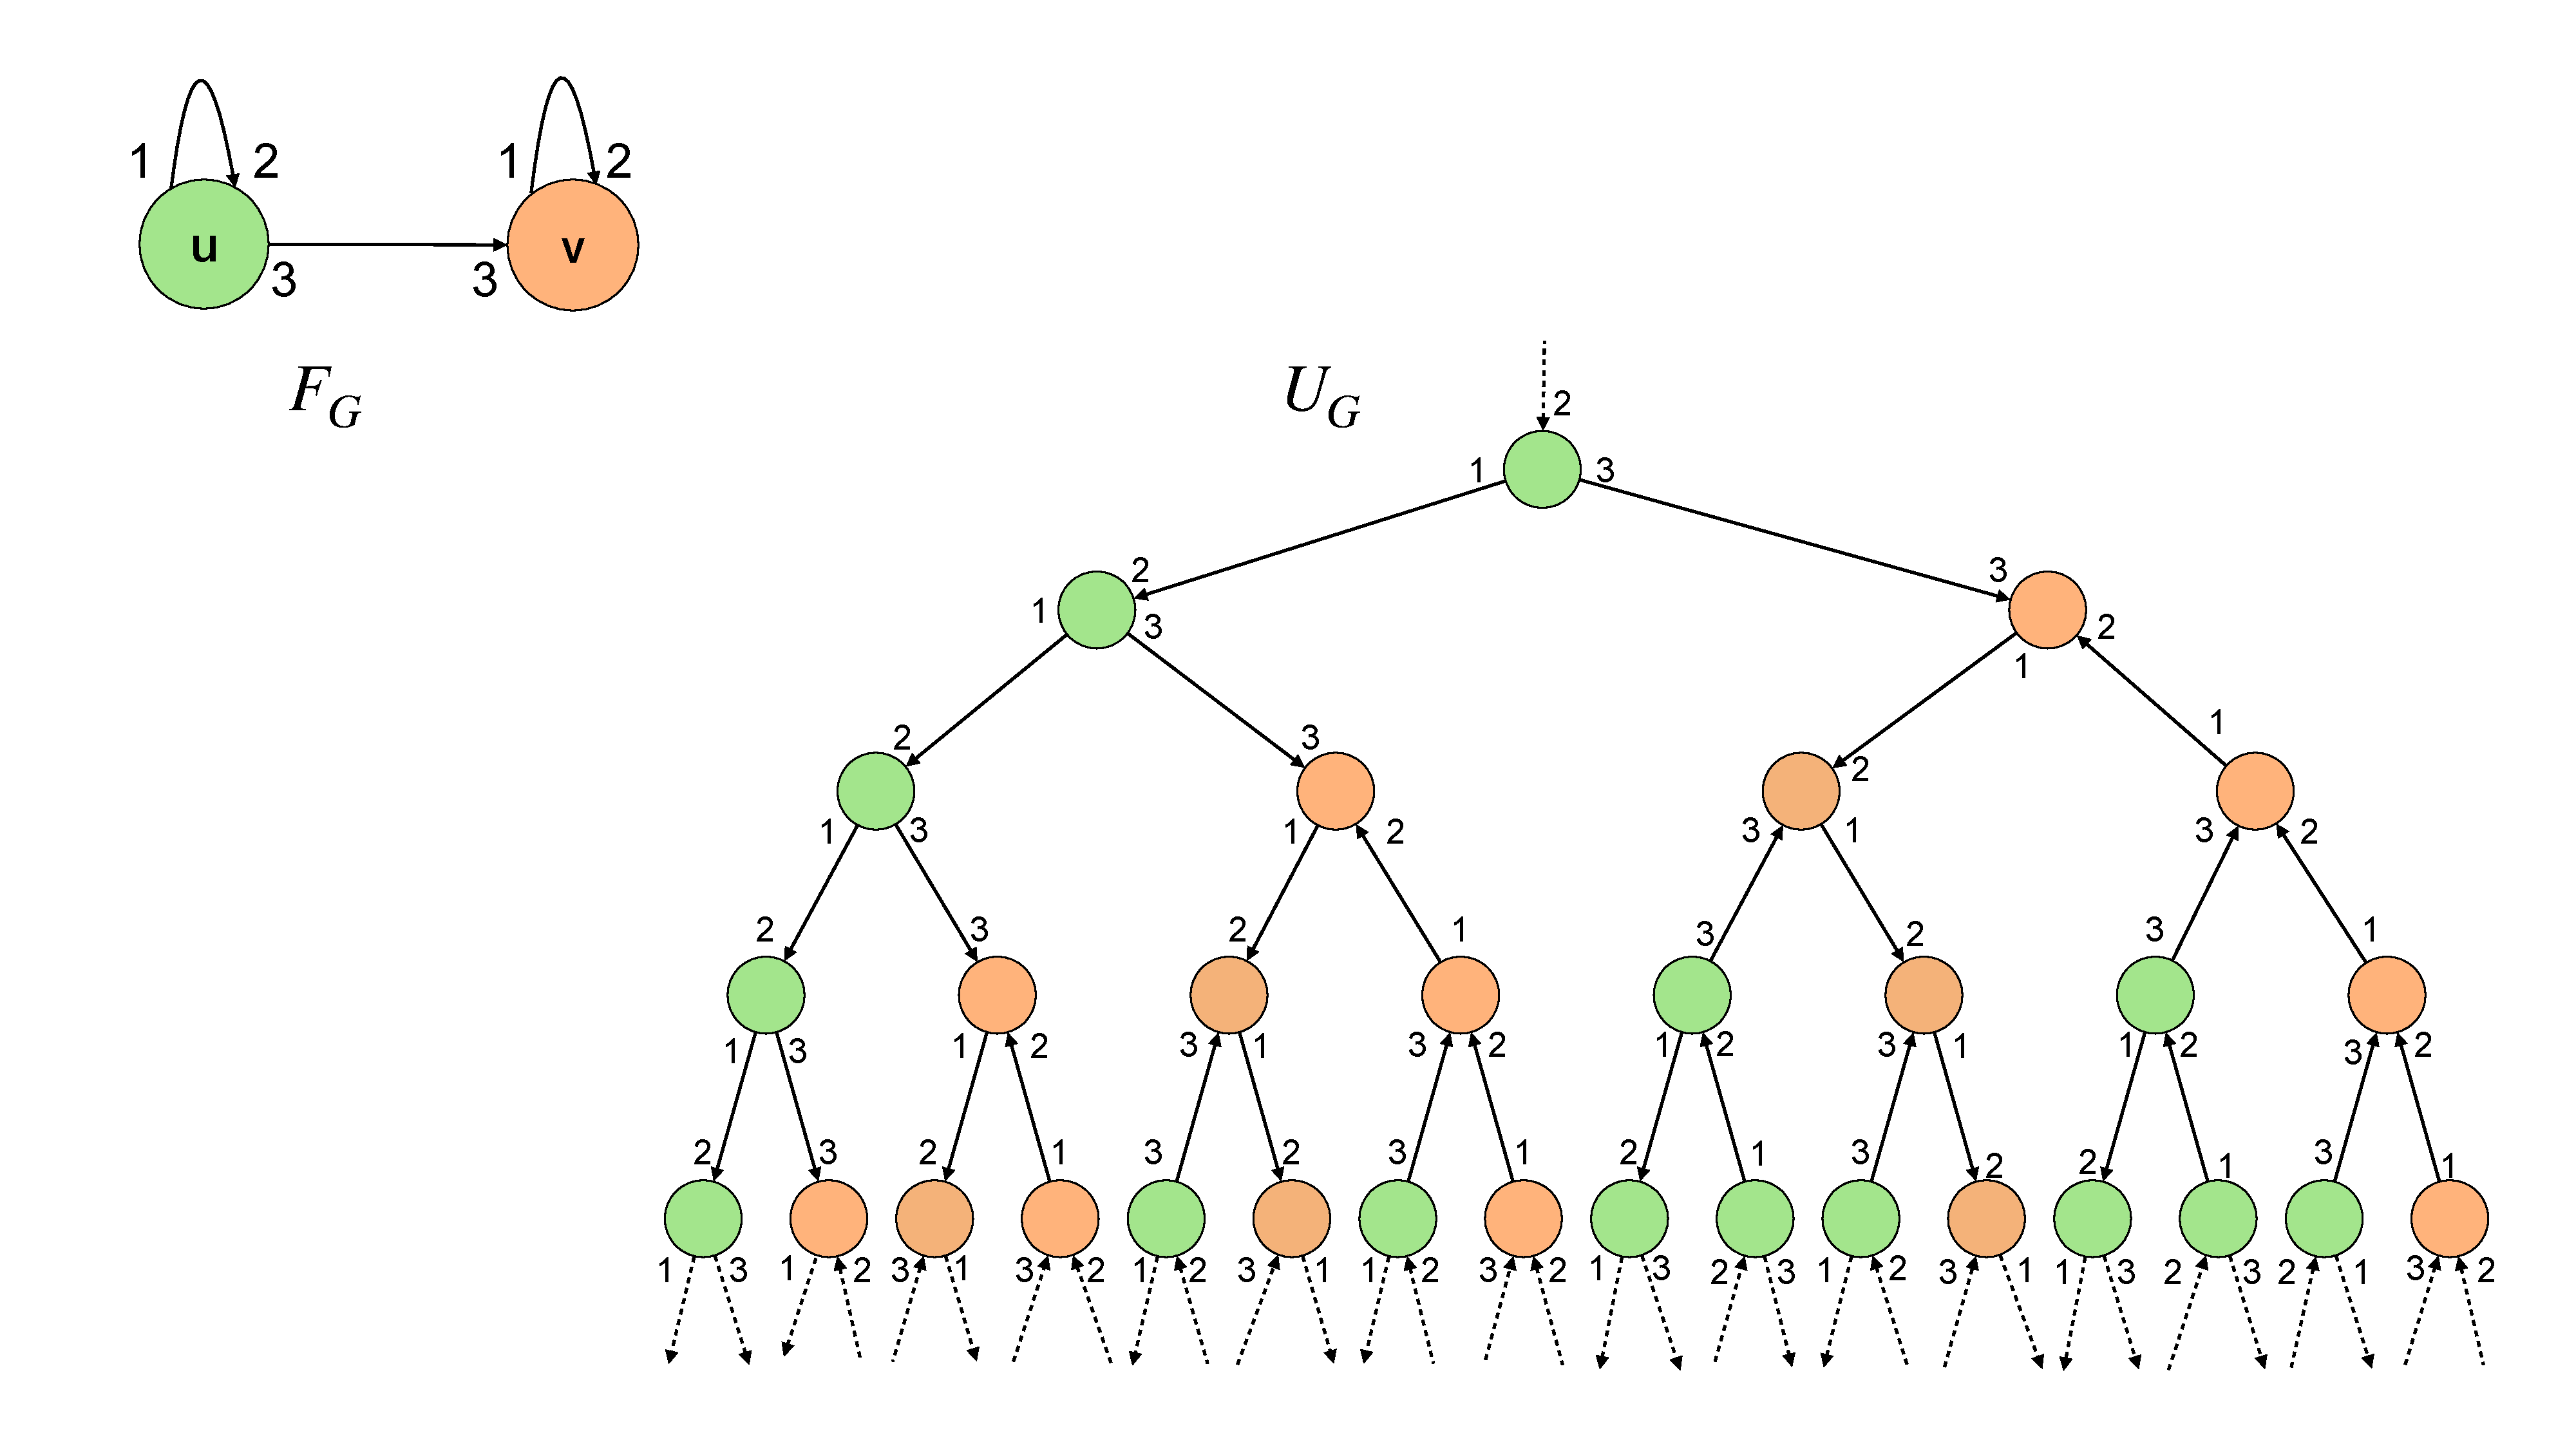
\includegraphics[scale = 0.22]{Figures/cover.pdf}
    \caption{$F_G$ and $U_G$}
    \label{fig:cv1}
\end{figure}

According to Jukka Suomela's textbook \cite{textbook}, we redefine here his definition of a covering map where the concerned graph's edges are oriented.
\begin{defi}
(Covering Map) Let $N = (V,P,p, \preceq)$ and $N' = (V',P',p',\preceq')$ be port-numbered networks whose edges are oriented, and let $\Phi: V \rightarrow V'$. We say that $\Phi$ is a covering map from $N$ to $N'$ if the following holds:
\begin{itemize}
    \item $\Phi$ is a surjection: $\Phi(V) = V'$
    \item $\Phi$ preserves degrees: $deg_N(v) = deg_{N'}(\Phi(v))$ for all $v \in V$.
    \item $\Phi$ preserves connections and port numbers: $p(u,i) = (v,j)$ implies
    $p'(\Phi(u), i) = (\Phi(v), j)$.
    \item $\Phi$ preserves orientations: $u \preceq v$ implies  $\Phi(u) \preceq' \Phi(v)$
\end{itemize}
\end{defi}
Theorem 8.1 of the textbook \cite[p.127]{textbook} also state that, if there exists a covering map $\Phi$ between two networks $N = (V,P,p, \preceq)$ and $N' = (V',P',p',\preceq')$, a deterministic algorithm that produce an output on $v \in V$ in $t=\mathcal{O}(1)$ must produce the same output for $v'\in V'$ after $t$ rounds if $v' = \Phi(v)$.\\\\
We now introduce $U_G = (V_U, E_U,\preceq_U)$ a tree that is the unfolded tree-like version of $F_G$ \cite[p. 7]{linear_in_delta} as in the figure \ref{fig:cv1}. We can see that a covering map between $F_G$ and $U_G$ exists.\\\\
 From this covering map, we know that :
 \begin{itemize}
     \item $A'$ must produce the same output for every node $u_i$ of $U_G$ that satisfy $u_i = \Phi(u)$
     \item $A'$ must produce the same output for every node $v_i$ of $U_G$ that satisfy $v_i = \Phi(v)$
 \end{itemize}
Hence, due to the port numbering of $F_G$, we can make the following requirements for $A'$ to produce a correct output:\\\\
$\exists u = (u_0,u_1,u_2),v = (v_0,v_1,v_2) \in W $ with $u_i,v_i\in \{A,B,C\}$ for $i\in \{0,1,2\}$ such that :
\begin{itemize}
    \item $\exists u_a,u_b \in u \hbox{ s.t. } (u_a,u_b)\in B$ with $a,b\in \{0,1,2\}, a\neq b$
    \item $\exists v_{a'},v_{b'} \in v \hbox{ s.t. } (v_{a'},v_{b'})\in B$ with $a',b'\in \{0,1,2\}, a'\neq b'$
    \item $(u_c,v_{c'})\in B$ where $c \in \{0,1,2\}$, $c\neq a, c\neq b$ and $c' \in \{0,1,2\}, c'\neq a', c'\neq b'$
\end{itemize}
In other words, for a node $u_i = \Phi(u)$ a configuration $u$ must exists such that $u_i$ can have 2 neighbors $u_a = \Phi(u)$ and $u_b = \Phi(u)$ and a neighbor $v_i = \Phi(v)$.
The sames goes for a node $v_i = \Phi(v)$ where a configuration $v$ must exists such that $v_i$ can have 2 neighbors $v_a = \Phi(v)$ and $v_b = \Phi(v)$ and a neighbor $u_i = \Phi(u)$.\\\\
If such requirements does not exists for a given problem, this implies that A' cannot have a correct output on $U_G$. By contraposition, $A$ must fails as well, we hence now that there exists a $log^*(n)$ lower bounds on the complexity of the problem.
\begin{exmp}
Let's take the following problem that encode the maximal independent set : $\Pi=(3,2,W,B)$ with :
\begin{itemize}
    \item $W = AAA, BBB, BBC, BCC$
    \item $B = AB, CC$
\end{itemize}
For each white configuration, let's check if it match the requirements for $u$ or $v$:
\begin{itemize}
    \item \textbf{AAA} : AA is not in $B$, hence, a node labelled with AAA cannot have any neighbors labelled with the same configuration.
    \item \textbf{AAA} : BB is not in $B$, hence, a node labelled with BBB cannot have any neighbors labelled with the same configuration.
    \item \textbf{BBC} : there is neither BB neither BC in $B$, again, BBC cannot have any neighbors labelled with the same configuration.
    \item \textbf{BCC} : Here we can see that $CC\in B$, let hence put that $u = BCC$ and $v = BCC$ since its the only configuration that allows a nodes to have 2 neighbors with the same configurations. however, we can see that $BB$ is not in $B$, a node of type $u$ cannot have a neighbor of type $v$. BCC is not fulfilling the requirements.
\end{itemize}
No configuration fulfill the requirements, the problem has a $log^*n$ lower bound.
\end{exmp}
